% Gated fusion (Table 5, panel C) — 구조 설명 그림. 빌드: tools/build_paper_figures.sh fig_gate_fusion
% 구현: experiments/실험12_융합방식_조건통일/exp_gate_oof.py --gate_inputs risk (게이트 입력 = 위험점수 2개)
% 색: 영상 #538EC6, 임상 #8C71BC, Cox #D8B24C (figstyle/fig2a 와 같은 계열), 게이트 #3A9D5D
\documentclass[border=4pt]{standalone}
\usepackage[T1]{fontenc}
\usepackage{newtxtext,newtxmath}
\usepackage{tikz}
\usetikzlibrary{arrows.meta}
\definecolor{imgc}{HTML}{538EC6}
\definecolor{clinc}{HTML}{8C71BC}
\definecolor{coxc}{HTML}{D8B24C}
\definecolor{gatec}{HTML}{3A9D5D}
\definecolor{ink}{HTML}{1F2A44}
\begin{document}
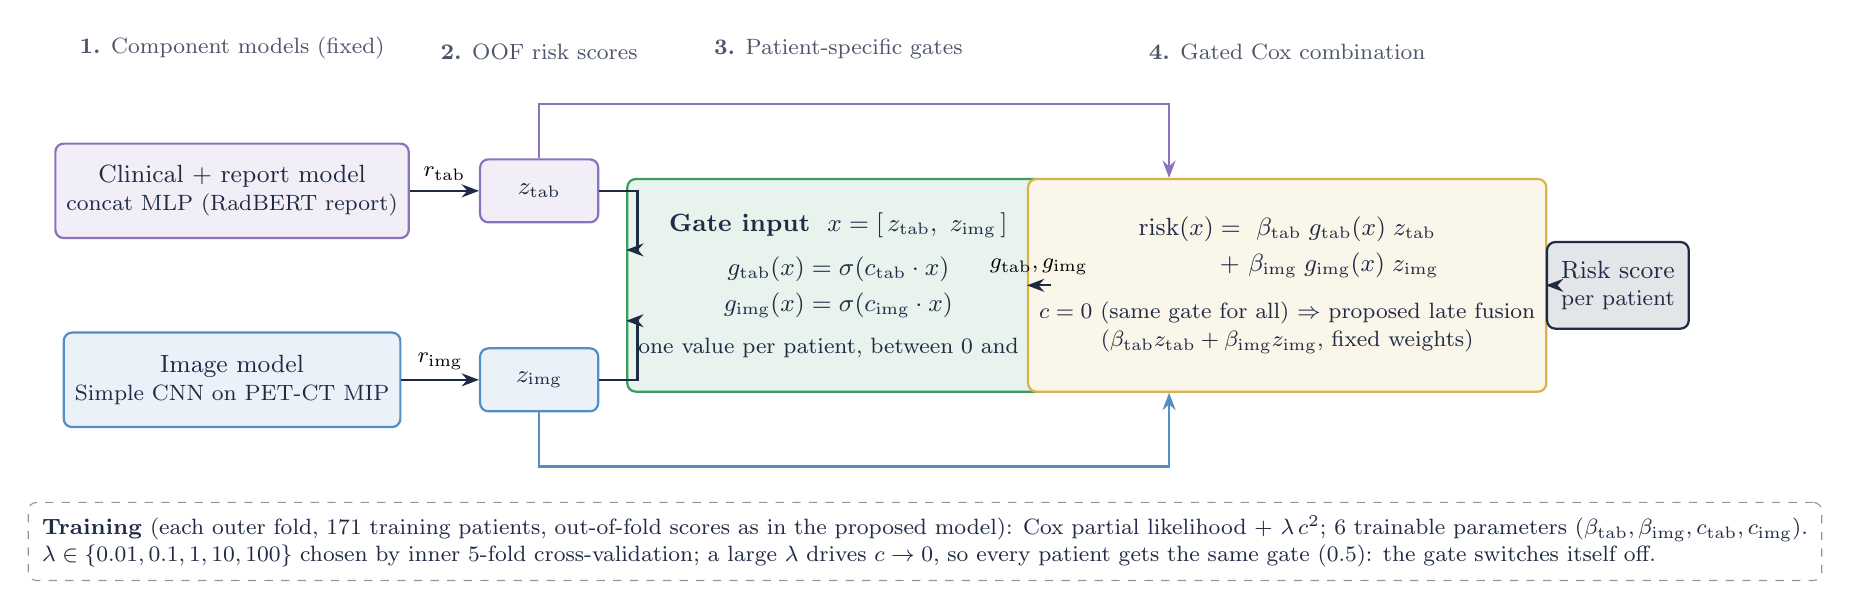
\begin{tikzpicture}[x=1cm, y=1cm, font=\small, >={Stealth[length=2.2mm]},
  box/.style={draw=#1, line width=0.8pt, rounded corners=3pt, fill=#1!12, align=center,
              inner sep=4pt, text=ink},
  arr/.style={->, line width=0.8pt, draw=ink},
  stagelbl/.style={font=\footnotesize, text=ink!80, align=center, anchor=south},
]
% ---- 단계 제목 (한 줄에 정렬) ----
\node[stagelbl] at (0,   2.75) {\textbf{1.} Component models (fixed)};
\node[stagelbl] at (3.9, 2.75) {\textbf{2.} OOF risk scores};
\node[stagelbl] at (7.7, 2.75) {\textbf{3.} Patient-specific gates};
\node[stagelbl] at (13.4,2.75) {\textbf{4.} Gated Cox combination};

% ---- 1. 고정된 두 축 모델 ----
\node[box=clinc, minimum width=38mm, minimum height=12mm] (tab) at (0, 1.2)
  {Clinical + report model\\[-1pt]{\footnotesize concat MLP (RadBERT report)}};
\node[box=imgc, minimum width=38mm, minimum height=12mm] (img) at (0,-1.2)
  {Image model\\[-1pt]{\footnotesize Simple CNN on PET-CT MIP}};

% ---- 2. 표준화한 OOF 위험점수 ----
\node[box=clinc, minimum width=15mm, minimum height=8mm] (zt) at (3.9, 1.2) {$z_{\mathrm{tab}}$};
\node[box=imgc,  minimum width=15mm, minimum height=8mm] (zi) at (3.9,-1.2) {$z_{\mathrm{img}}$};
\draw[arr] (tab) -- node[font=\footnotesize, above] {$r_{\mathrm{tab}}$} (zt);
\draw[arr] (img) -- node[font=\footnotesize, above] {$r_{\mathrm{img}}$} (zi);

% ---- 3. 게이트 ----
\node[box=gatec, minimum width=42mm, minimum height=27mm] (gate) at (7.7, 0)
  {\textbf{Gate input} \ $x = [\,z_{\mathrm{tab}},\ z_{\mathrm{img}}\,]$\\[5pt]
   $g_{\mathrm{tab}}(x) = \sigma(c_{\mathrm{tab}}\cdot x)$\\[2pt]
   $g_{\mathrm{img}}(x) = \sigma(c_{\mathrm{img}}\cdot x)$\\[4pt]
   {\footnotesize one value per patient, between 0 and 1}};
\draw[arr] (zt.east) -- (5.15, 1.2) -- (5.15, 0.45) -- (gate.west |- 0,0.45);
\draw[arr] (zi.east) -- (5.15,-1.2) -- (5.15,-0.45) -- (gate.west |- 0,-0.45);

% ---- 4. 결합 ----
\node[box=coxc, minimum width=50mm, minimum height=27mm] (comb) at (13.4, 0)
  {$\mathrm{risk}(x) =\ \beta_{\mathrm{tab}}\; g_{\mathrm{tab}}(x)\; z_{\mathrm{tab}}$\\[2pt]
   $\qquad\quad\; +\ \beta_{\mathrm{img}}\; g_{\mathrm{img}}(x)\; z_{\mathrm{img}}$\\[6pt]
   {\footnotesize $c = 0$ (same gate for all) $\Rightarrow$ proposed late fusion}\\[-1pt]
   {\footnotesize ($\beta_{\mathrm{tab}} z_{\mathrm{tab}} + \beta_{\mathrm{img}} z_{\mathrm{img}}$, fixed weights)}};
\draw[arr] (gate) -- node[font=\footnotesize, above] {$g_{\mathrm{tab}}, g_{\mathrm{img}}$} (comb);
% 위험점수 자체도 결합 단계로 들어간다 (위·아래로 돌아서)
\draw[arr, draw=clinc] (zt.north) -- (3.9, 2.3) -- (11.9, 2.3) -- (11.9,0 |- comb.north);
\draw[arr, draw=imgc]  (zi.south) -- (3.9,-2.3) -- (11.9,-2.3) -- (11.9,0 |- comb.south);

% ---- 출력 ----
\node[box=ink, minimum width=18mm, minimum height=11mm] (out) at (17.6, 0)
  {Risk score\\[-1pt]{\footnotesize per patient}};
\draw[arr] (comb) -- (out);

% ---- 학습 ----
\node[draw=ink!50, dashed, rounded corners=3pt, align=left, font=\footnotesize, text=ink,
      inner sep=5pt, anchor=north] at (8.8,-2.75)
  {\textbf{Training} (each outer fold, 171 training patients, out-of-fold scores as in the proposed model):
   Cox partial likelihood $+\ \lambda\,\lVert c\rVert^{2}$;\
   6 trainable parameters ($\beta_{\mathrm{tab}}, \beta_{\mathrm{img}}, c_{\mathrm{tab}}, c_{\mathrm{img}}$).\\
   $\lambda \in \{0.01, 0.1, 1, 10, 100\}$ chosen by inner 5-fold cross-validation;
   a large $\lambda$ drives $c \to 0$, so every patient gets the same gate (0.5): the gate switches itself off.};
\end{tikzpicture}
\end{document}
